\PassOptionsToPackage{table}{xcolor}
\documentclass[10pt, aspectratio=169]{beamer}

\usetheme{metropolis}
\usepackage{fontspec}
\usepackage{fontawesome5}
\usepackage{booktabs}
\usepackage{tikz}
\usetikzlibrary{arrows.meta,positioning}
\usepackage{xcolor}
\usepackage{graphicx}
\usepackage{capt-of}
\usepackage{amsmath}
\usepackage{amssymb}
\usepackage{siunitx}

% University of Florence inspired palette (WCAG-friendly)
\definecolor{QuantumTeal}{HTML}{2F4858}
\definecolor{QuantumBlue}{HTML}{A51E2D}
\definecolor{SuccessGreen}{HTML}{1F6F50}
\definecolor{AlertRed}{HTML}{8F1D21}
\definecolor{FillCPU}{RGB}{242,244,247}
\definecolor{FillGPU}{RGB}{224,236,247}
\definecolor{FillCUDA}{RGB}{226,242,233}
\definecolor{FillSVM}{RGB}{233,245,233}

\setbeamercolor{normal text}{fg=black, bg=white}
\setbeamercolor{frametitle}{bg=QuantumBlue, fg=white}
\setbeamercolor{title separator}{fg=QuantumTeal}
\setbeamercolor{progress bar}{fg=QuantumTeal, bg=gray!25}
\setbeamercolor{alerted text}{fg=AlertRed}
\setbeamercolor{block title}{bg=QuantumBlue, fg=white}
\setbeamercolor{block body}{bg=gray!8, fg=black}
\setbeamercolor{block title alerted}{bg=AlertRed, fg=white}
\setbeamercolor{block body alerted}{bg=gray!8, fg=black}
\setbeamercolor{block title example}{bg=SuccessGreen, fg=white}
\setbeamercolor{block body example}{bg=gray!8, fg=black}

\title{Acceleration of Quantum Kernel Methods\\for Image Classification Tasks}
\subtitle{Project Work Parallel Programming}
\date{}
\author{\textbf{Fouepe Dylan}}
\institute{\faUniversity\ University of Florence\\\faAtom\ Parallel Programming -- 2025}

\begin{document}
\begin{frame}[plain]
    \centering
    \vspace*{0.9cm}
    {\usebeamerfont{title}\usebeamercolor[fg]{title}\inserttitle\par}
    \vspace{0.45cm}
    {\usebeamerfont{subtitle}\usebeamercolor[fg]{subtitle}\insertsubtitle\par}
    \vfill
    {\large\textbf{\insertauthor}\par}
    \vspace{0.25cm}
    {\normalsize\insertinstitute\par}
    \vspace*{0.65cm}
\end{frame}

\begin{frame}{Overview}
    \setbeamertemplate{section in toc}[sections numbered]
    \tableofcontents[hideallsubsections]
\end{frame}

% =========================================================================
\section{Context \& Scope}
% =========================================================================

\begin{frame}{Context \& Motivation}
    \begin{columns}[T,onlytextwidth]
        \column{0.52\textwidth}
        \textbf{\faLightbulb\ Quantum Kernel SVMs}
        \begin{itemize}
            \item Project classical data into a $2^Q$-dimensional Hilbert space.
            \item Fidelity kernel: $k(x_i,x_j) = |\langle\psi(x_i)|\psi(x_j)\rangle|^2$.
            \item At $Q=16$: $65{,}536$ complex amplitudes per state.
            \item Guaranteed convex SVM optimization.
        \end{itemize}
        \vspace{0.2cm}
        \textbf{\faExclamationTriangle\ HPC Bottleneck}
        \begin{itemize}
            \item Gram matrix cost: $\mathcal{O}(N^2 \cdot 2^Q)$.
            \item GPU/CUDA acceleration is essential at scale.
        \end{itemize}
        \column{0.45\textwidth}
        \begin{block}{\faBullseye\ Three Research Questions}
            \begin{enumerate}
                \item How do classical and quantum-kernel SVMs compare on the same binary tasks?
                \item Which backend offers the best throughput--runtime trade-off at 16 qubits?
                \item Which empirical signals indicate kernel concentration?
            \end{enumerate}
        \end{block}
    \end{columns}
\end{frame}

% =========================================================================
\section{Experimental Methodology}
% =========================================================================

\begin{frame}{Datasets \& Binary Tasks}
    \begin{columns}[T,onlytextwidth]
        \column{0.50\textwidth}
        Three datasets, binarized into three difficulty levels:
        \vspace{0.3cm}

        \small
        \rowcolors{2}{gray!10}{white}
        \begin{tabular}{llll}
            \toprule
            \textbf{Dataset} & \textbf{Easy} & \textbf{Med} & \textbf{Hard} \\
            \midrule
            Fashion-MNIST & 0 vs 1 & 3 vs 8 & 0 vs 6 \\
            CIFAR-10      & 1 vs 6 & 0 vs 2 & 3 vs 5 \\
            SVHN          & 1 vs 0 & 2 vs 7 & 3 vs 5 \\
            \bottomrule
        \end{tabular}
        \column{0.47\textwidth}
        \begin{block}{\faFlask\ Default Setup}
            \begin{itemize}
                \item $Q = 16$ qubits $\to 2^{16}$ amplitudes
                \item \textbf{YZ ansatz} with entangling layers (fixed weights)
                \item 3-fold CV + Optuna for hyperparameter $C$
                \item Metrics: F1, AUC, runtime, SV fraction, kernel std
            \end{itemize}
        \end{block}
    \end{columns}
\end{frame}

\begin{frame}{Preprocessing Pipeline \& Fidelity Kernel}
    \begin{columns}[T,onlytextwidth]
        \column{0.48\textwidth}
        \textbf{Feature pipeline:}
        \begin{enumerate}
            \item Extract pixels and flatten
            \item PCA to $d=16$ components
            \item Range scaling
            \item Encode via \textit{angle map}, \textit{Y map} or \textit{YZ map}
            \item Simulate states via PennyLane
        \end{enumerate}
        \vspace{0.2cm}
        \textbf{Fidelity kernel:}
        \[K_{ij} = \left|\sum_{k=1}^{2^Q} S_A[i,k]\,\overline{S_B[j,k]}\right|^2\]
        \column{0.48\textwidth}
        \textbf{Training protocol:}
        \begin{itemize}
            \item Train/test split from dataset
            \item 3-fold CV on training partition
            \item Hyperparameter search ($C$) via Optuna
            \item Final re-fit on train+val, eval on test set
        \end{itemize}
        \vspace{0.2cm}
        \begin{alertblock}{\faInfoCircle\ Kernel-based, not variational}
            Weights are fixed at init -- kernel method, not a training loop.
        \end{alertblock}
    \end{columns}
\end{frame}

% =========================================================================
\section{HPC Architecture}
% =========================================================================

\begin{frame}{Unified Backend API}
    \begin{columns}[T,onlytextwidth]
        \column{0.44\textwidth}
        Three execution paths, same normalization and SVM:
        \begin{itemize}
            \item \textbf{CPU base} -- NumPy reference, no VRAM tiling
            \item \textbf{GPU base} -- PyTorch GPU matmul + pinned memory + CUDA streams
            \item \textbf{GPU custom} -- PyTorch states $\to$ DLPack $\to$ CuPy $\to$ custom CUDA kernel (FP64)
        \end{itemize}
        \vspace{0.2cm}
        {\small SVM solver always runs on CPU.}
        \column{0.53\textwidth}
        \begin{center}
        \resizebox{0.97\linewidth}{!}{%
        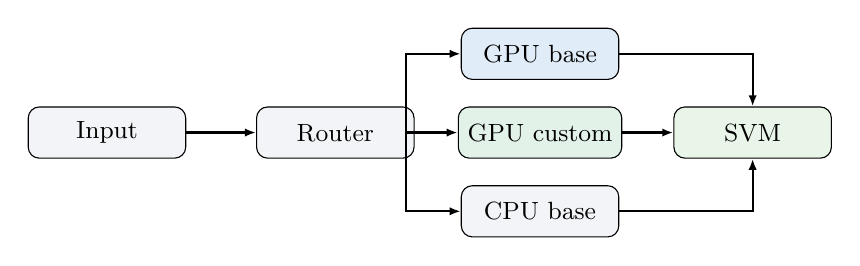
\begin{tikzpicture}[
            box/.style={draw, rounded corners, minimum width=2.0cm, minimum height=0.65cm, align=center, font=\small},
            arr/.style={-{Latex[length=4pt]}, thick}
        ]
            \node[box, fill=FillCPU]  (data)  at (0,0)      {Input};
            \node[box, fill=FillCPU]  (route) at (2.9,0)    {Router};
            \node[box, fill=FillGPU]  (gpub)  at (5.5,1.0)  {GPU base};
            \node[box, fill=FillCUDA] (gpuc)  at (5.5,0)    {GPU custom};
            \node[box, fill=FillCPU]  (cpu)   at (5.5,-1.0) {CPU base};
            \node[box, fill=FillSVM]  (svm)   at (8.2,0)    {SVM};
            \draw[arr] (data) -- (route);
            \draw[arr] (route) -- ++(0.9,0) |- (gpub);
            \draw[arr] (route) -- (gpuc);
            \draw[arr] (route) -- ++(0.9,0) |- (cpu);
            \draw[arr] (gpub) -| (svm);
            \draw[arr] (gpuc) -- (svm);
            \draw[arr] (cpu)  -| (svm);
        \end{tikzpicture}%
        }
        \end{center}
    \end{columns}
\end{frame}

\begin{frame}{Backend Optimizations \& Shared Normalization}
    \begin{columns}[T,onlytextwidth]
        \column{0.48\textwidth}
        \textbf{Key optimizations:}
        \begin{itemize}
            \item \textbf{VRAM-aware tiling}: block size auto-tuned to budget
            \item \textbf{Kernel autotuning}: tile sizes cached persistently
            \item \textbf{Bulk precompute}: states prebuilt when memory allows
            \item \textbf{Stream pool}: CUDA stream orchestration
            \item Best: vram\_fraction=0.95, num\_streams=1, GPU base pinned+streams
        \end{itemize}
        \column{0.48\textwidth}
        \begin{block}{\faBalanceScale\ Shared Normalization}
            All backends use identical post-processing:
            \[\hat{K}_{ij} = \frac{K(X,Y)_{ij}}{\sqrt{K(X,X)_{ii}\,K(Y,Y)_{jj}}}\]
            \begin{itemize}
                \item NaN/Inf checks before writing
                \item Diagonal validation before SVM fit
                \item Guarantees fair comparison
            \end{itemize}
        \end{block}
    \end{columns}
\end{frame}

\begin{frame}{GPU Custom: Kernel Construction Pipeline}
\begin{center}
\resizebox{0.90\linewidth}{!}{%
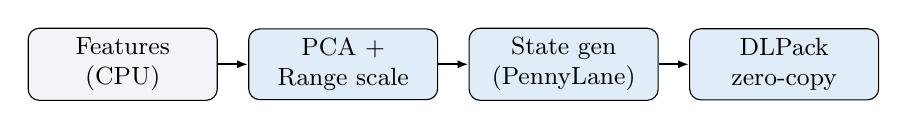
\begin{tikzpicture}[
    host/.style={draw, rounded corners, fill=FillGPU, minimum width=2.4cm, minimum height=0.7cm, align=center, font=\small},
    io/.style={draw, rounded corners, fill=FillCPU, minimum width=2.4cm, minimum height=0.7cm, align=center, font=\small},
    arr/.style={-{Latex[length=4pt]}, thick},
    note/.style={font=\scriptsize, align=center}
]

%% ---- HOST SIDE (top row) ----
\node[io]   (feat)    at (0, 0)     {Features\\(CPU)};
\node[host] (pca)     at (2.8, 0)   {PCA +\\Range scale};
\node[host] (state)   at (5.6, 0)   {State gen\\(PennyLane)};
\node[host] (dlpack)  at (8.4, 0)   {DLPack\\zero-copy};

%% ---- ARROWS host flow ----
\draw[arr] (feat)   -- (pca);
\draw[arr] (pca)    -- (state);
\draw[arr] (state)  -- (dlpack);

\end{tikzpicture}%
}
\end{center}
    \begin{columns}[T,onlytextwidth]
        \column{0.48\textwidth}
        \textbf{Host preprocessing (step 1/3):}
        \begin{itemize}
            \item Raw image pixels extracted and flattened
            \item PCA to 16 components + range scaling
            \item Quantum states generated via PennyLane in \textbf{FP64}
            \item Output: complex state matrix $S \in \mathbb{C}^{N \times 2^Q}$
        \end{itemize}
        \column{0.48\textwidth}
        \begin{exampleblock}{Why FP64?}
            FP32 leads to \textbf{kernel collapse} ($AUC \approx 0.5$) due to floating-point cancellation in the fidelity dot products at $2^{16}$ dimensions.
        \end{exampleblock}
    \end{columns}
\end{frame}

\begin{frame}{GPU Custom: Control \& Cache Layer (2/3)}
    \begin{center}
    \resizebox{0.90\linewidth}{!}{%
        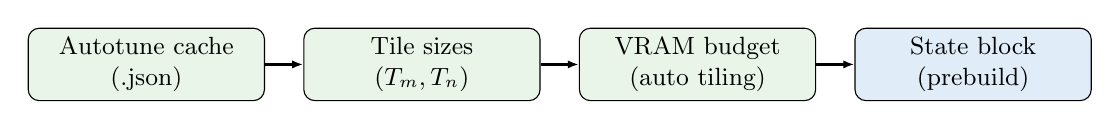
\begin{tikzpicture}[
            cache/.style={draw, rounded corners, fill=FillSVM, minimum width=3.0cm, minimum height=0.75cm, align=center, font=\small},
            host/.style={draw, rounded corners, fill=FillGPU, minimum width=3.0cm, minimum height=0.75cm, align=center, font=\small},
            arr/.style={-{Latex[length=4pt]}, thick}
        ]
            \node[cache] (autocache) at (0.0,  0) {Autotune cache\\(.json)};
            \node[cache] (tiles)     at (3.5,  0) {Tile sizes\\$(T_m, T_n)$};
            \node[cache] (vram)      at (7.0,  0) {VRAM budget\\(auto tiling)};
            \node[host]  (stateblk)  at (10.5, 0) {State block\\(prebuild)};
            \draw[arr] (autocache) -- (tiles);
            \draw[arr] (tiles)     -- (vram);
            \draw[arr] (vram)      -- (stateblk);
        \end{tikzpicture}%
    }
    \end{center}
    \vspace{0.25cm}
    \small
    \textbf{How the control layer works:}
    \begin{itemize}
        \setlength\itemsep{0.25em}
        \item \textbf{Autotune cache}: tile sizes $(T_m,T_n)$ measured once per (nq, dtype) and saved to JSON
        \item \textbf{VRAM-aware tiling}: vram\_fraction=0.95 caps state block size to available GPU memory
        \item \textbf{Bulk precompute}: if the full block fits, states are prebuilt to reduce PennyLane round-trips
        \item Optimal profile in benchmarks: \textbf{1 stream} with \textbf{pinned memory} (GPU base path)
    \end{itemize}
\end{frame}

\begin{frame}{GPU Custom: Device Core (3/3)}
    \begin{center}
    \resizebox{0.90\linewidth}{!}{%
        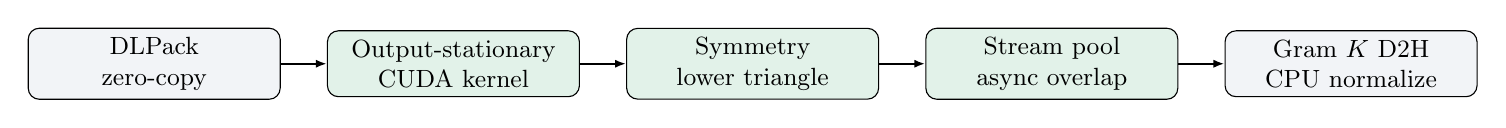
\begin{tikzpicture}[
            dev/.style={draw, rounded corners, fill=FillCUDA, minimum width=3.2cm, minimum height=0.75cm, align=center, font=\small},
            io/.style={draw, rounded corners, fill=FillCPU, minimum width=3.2cm, minimum height=0.75cm, align=center, font=\small},
            arr/.style={-{Latex[length=4pt]}, thick}
        ]
            \node[io]  (dlpack)  at (0.0, 0)  {DLPack\\zero-copy};
            \node[dev] (kernel)  at (3.8, 0)  {Output-stationary\\CUDA kernel};
            \node[dev] (sym)     at (7.6, 0)  {Symmetry\\lower triangle};
            \node[dev] (stream)  at (11.4,0)  {Stream pool\\async overlap};
            \node[io]  (gram)    at (15.2,0)  {Gram $K$ D2H\\CPU normalize};
            \draw[arr] (dlpack) -- (kernel);
            \draw[arr] (kernel) -- (sym);
            \draw[arr] (sym)    -- (stream);
            \draw[arr] (stream) -- (gram);
        \end{tikzpicture}%
    }
    \end{center}
    \vspace{0.2cm}
    \small
    \textbf{Device execution:}
    \begin{itemize}
        \setlength\itemsep{0.20em}
        \item \textbf{DLPack}: PyTorch GPU tensor $\to$ CuPy with \textbf{zero memory copy}
        \item \textbf{Output-stationary}: each CUDA thread writes exactly one $K_{ij}$ (no write conflicts)
        \item \textbf{Symmetry}: lower triangle only; then $K_{ji} \gets K_{ij}$ mirrors upper entries
        \item \textbf{Stream pool}: asynchronous block overlap between state prep and Gram compute
        \item Final step: D2H transfer of $K$ and CPU-side cross-normalization
    \end{itemize}
\end{frame}

% =========================================================================
\section{Performance Benchmark}
% =========================================================================

\begin{frame}{Throughput by Dataset \& Backend (Mpairs/s)}
    \begin{center}
    {\scriptsize Highest qubit setting per dataset (Fashion: 12 qubits; CIFAR-10/SVHN: 16 qubits)}
    \end{center}
    \vspace{-0.15cm}
    \begin{center}
    \scriptsize
    \rowcolors{2}{gray!10}{white}
    \begin{tabular}{llcccc}
        \toprule
        \textbf{Dataset} & \textbf{Size} & \textbf{Qubits} & \textbf{CPU base} & \textbf{GPU base} & \textbf{GPU custom} \\
        \midrule
        fashion & 256  & 12 & 0.0059 & 0.0140 & \textbf{0.0159} \\
        fashion & 512  & 12 & 0.0224 & \textbf{0.0299} & 0.0298 \\
        fashion & 1024 & 12 & \textbf{0.0856} & 0.0575 & 0.0546 \\
        cifar10 & 256  & 16 & 0.0020 & 0.0057 & \textbf{0.0062} \\
        cifar10 & 512  & 16 & 0.0086 & \textbf{0.0175} & 0.0112 \\
        cifar10 & 1024 & 16 & 0.0319 & \textbf{0.0375} & 0.0245 \\
        svhn    & 256  & 16 & 0.0023 & 0.0053 & \textbf{0.0058} \\
        svhn    & 512  & 16 & 0.0097 & \textbf{0.0175} & 0.0124 \\
        svhn    & 1024 & 16 & 0.0328 & \textbf{0.0366} & 0.0243 \\
        \bottomrule
    \end{tabular}
    \end{center}
    \vspace{0.1cm}
    {\small At size 256: GPU backends dominate. \ At size 512: GPU base fastest. \ At size 1024: CPU base recovers on Fashion.}
\end{frame}

\begin{frame}{Benchmark Profile -- Fashion-MNIST}
    \begin{center}
        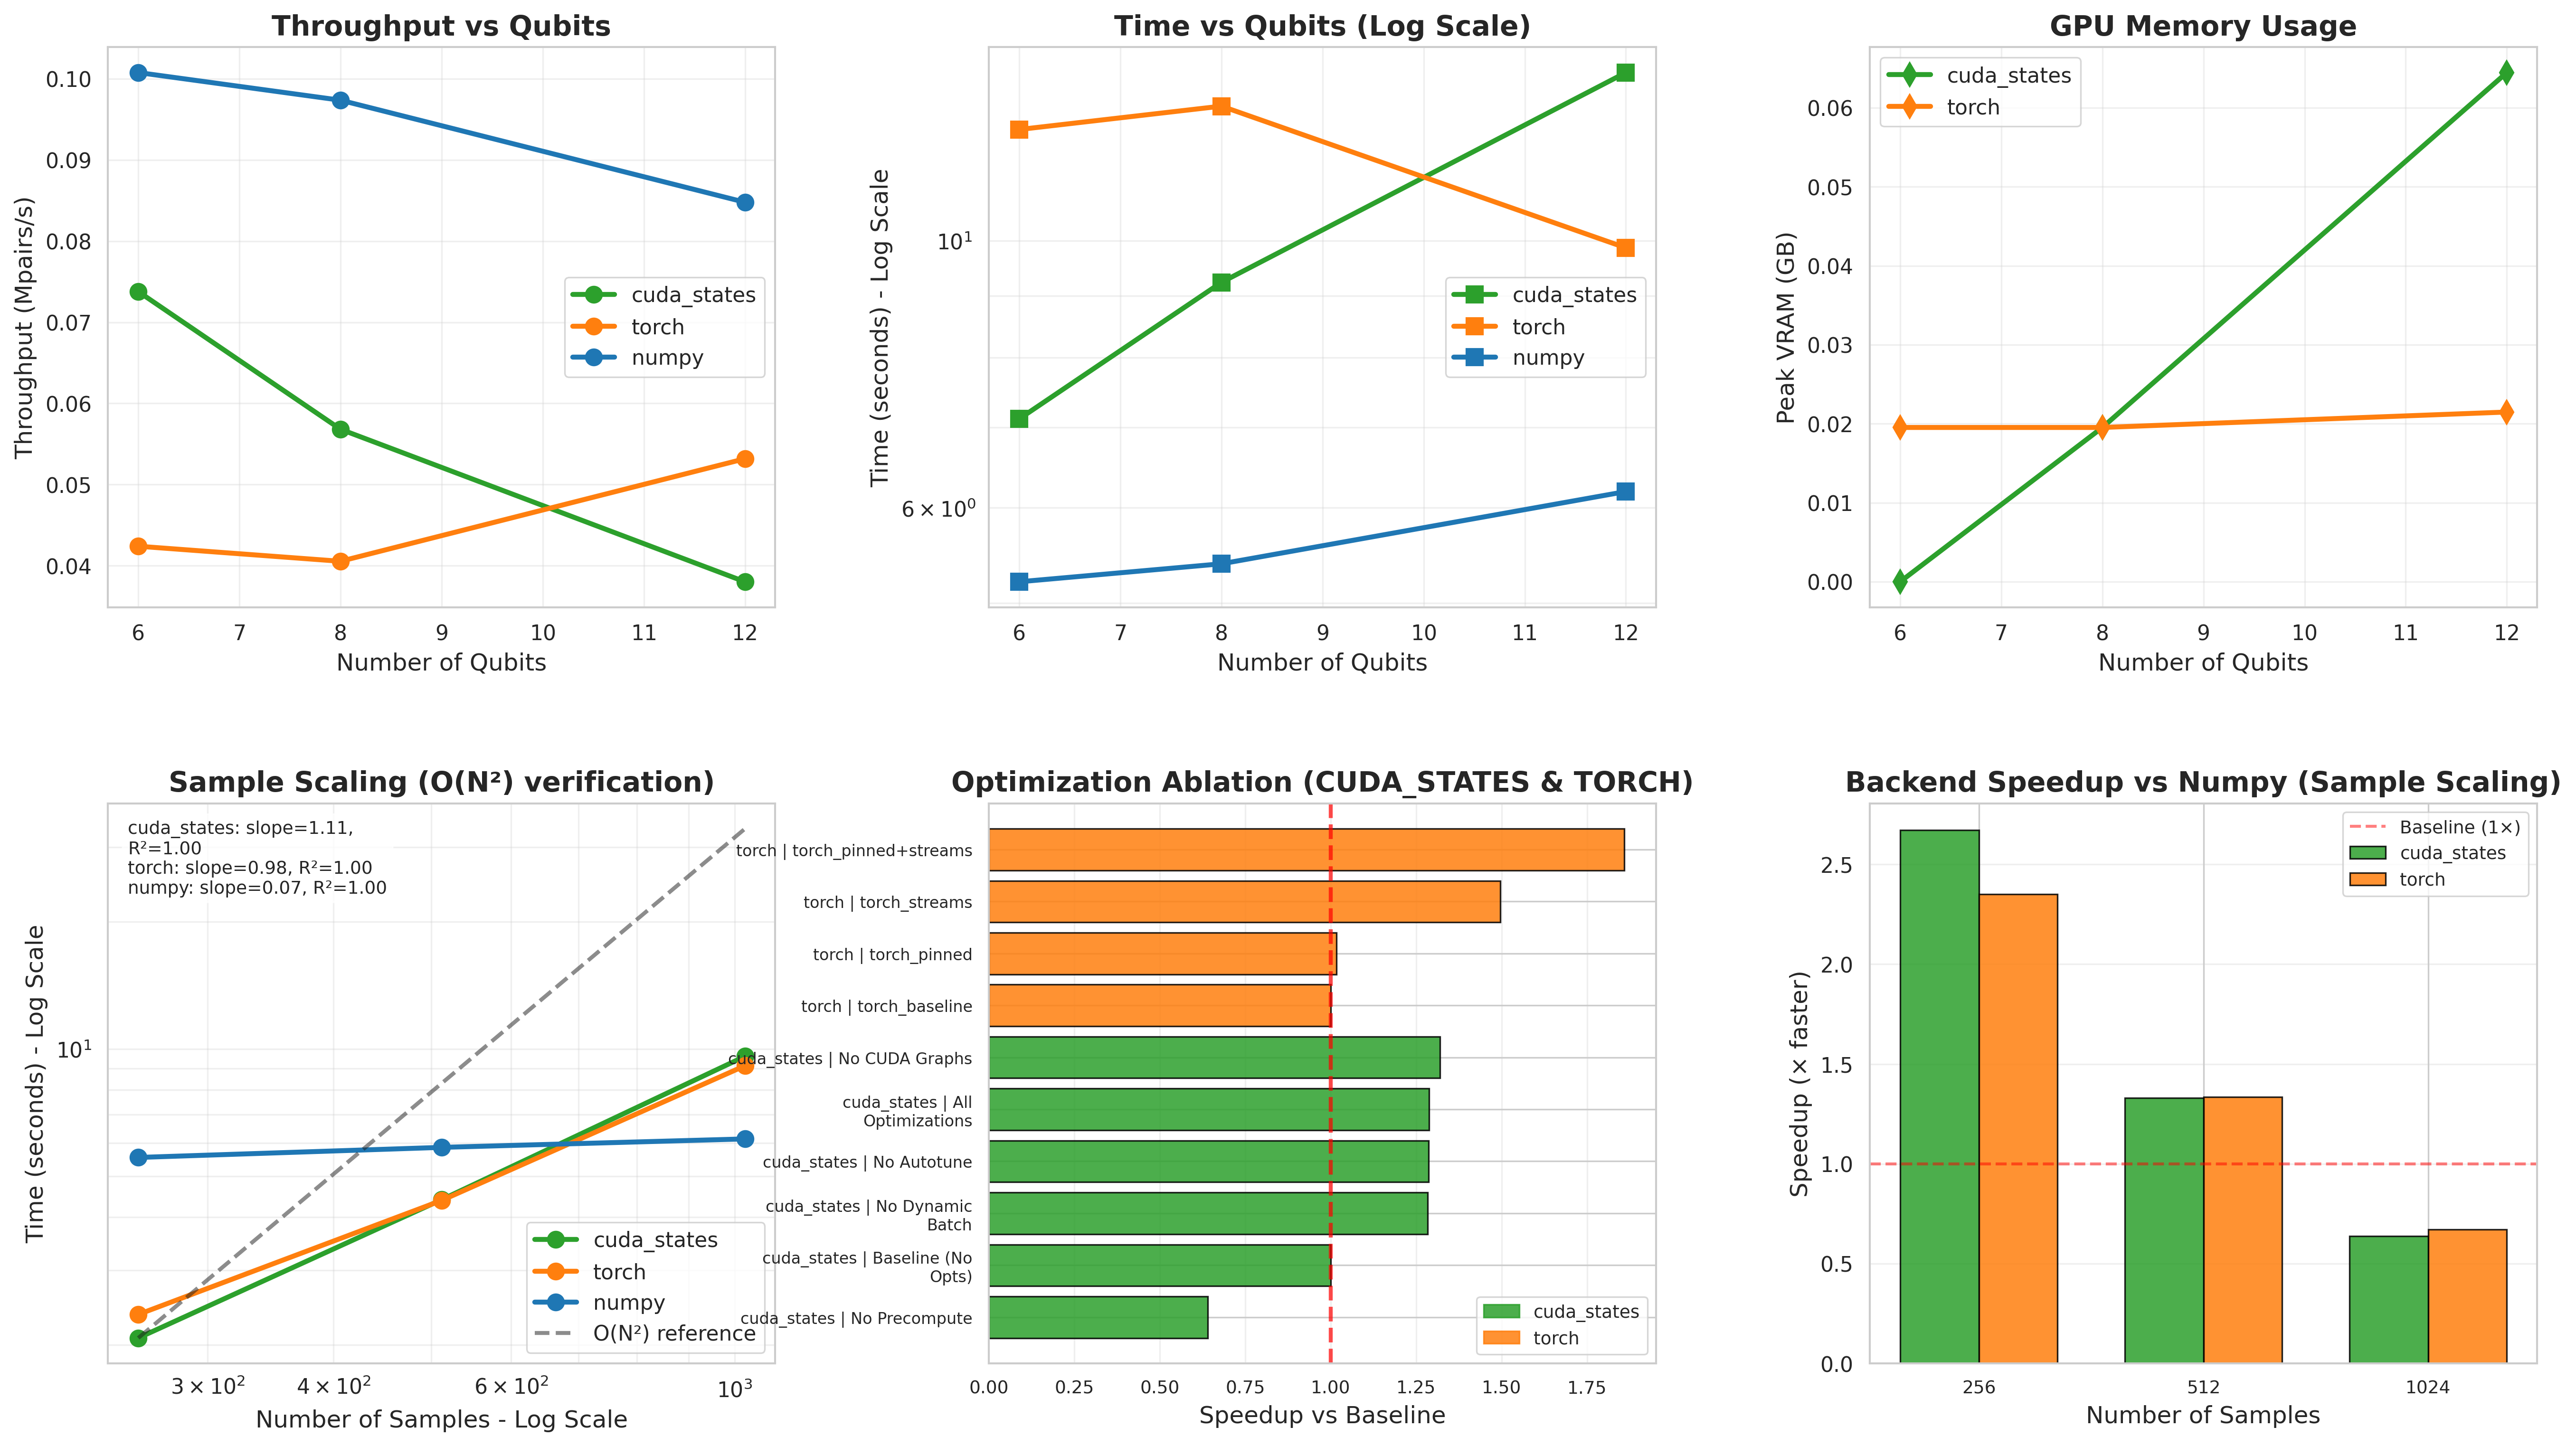
\includegraphics[width=0.72\textwidth]{benchmark_results/fashion/benchmark.png}
    \end{center}
    {\scriptsize Backend ranking is \textbf{not global}: it varies with sample size and dataset profile.}
\end{frame}

\begin{frame}{Benchmark Profiles -- CIFAR-10 \& SVHN}
    \begin{columns}[T,onlytextwidth]
        \column{0.50\textwidth}
        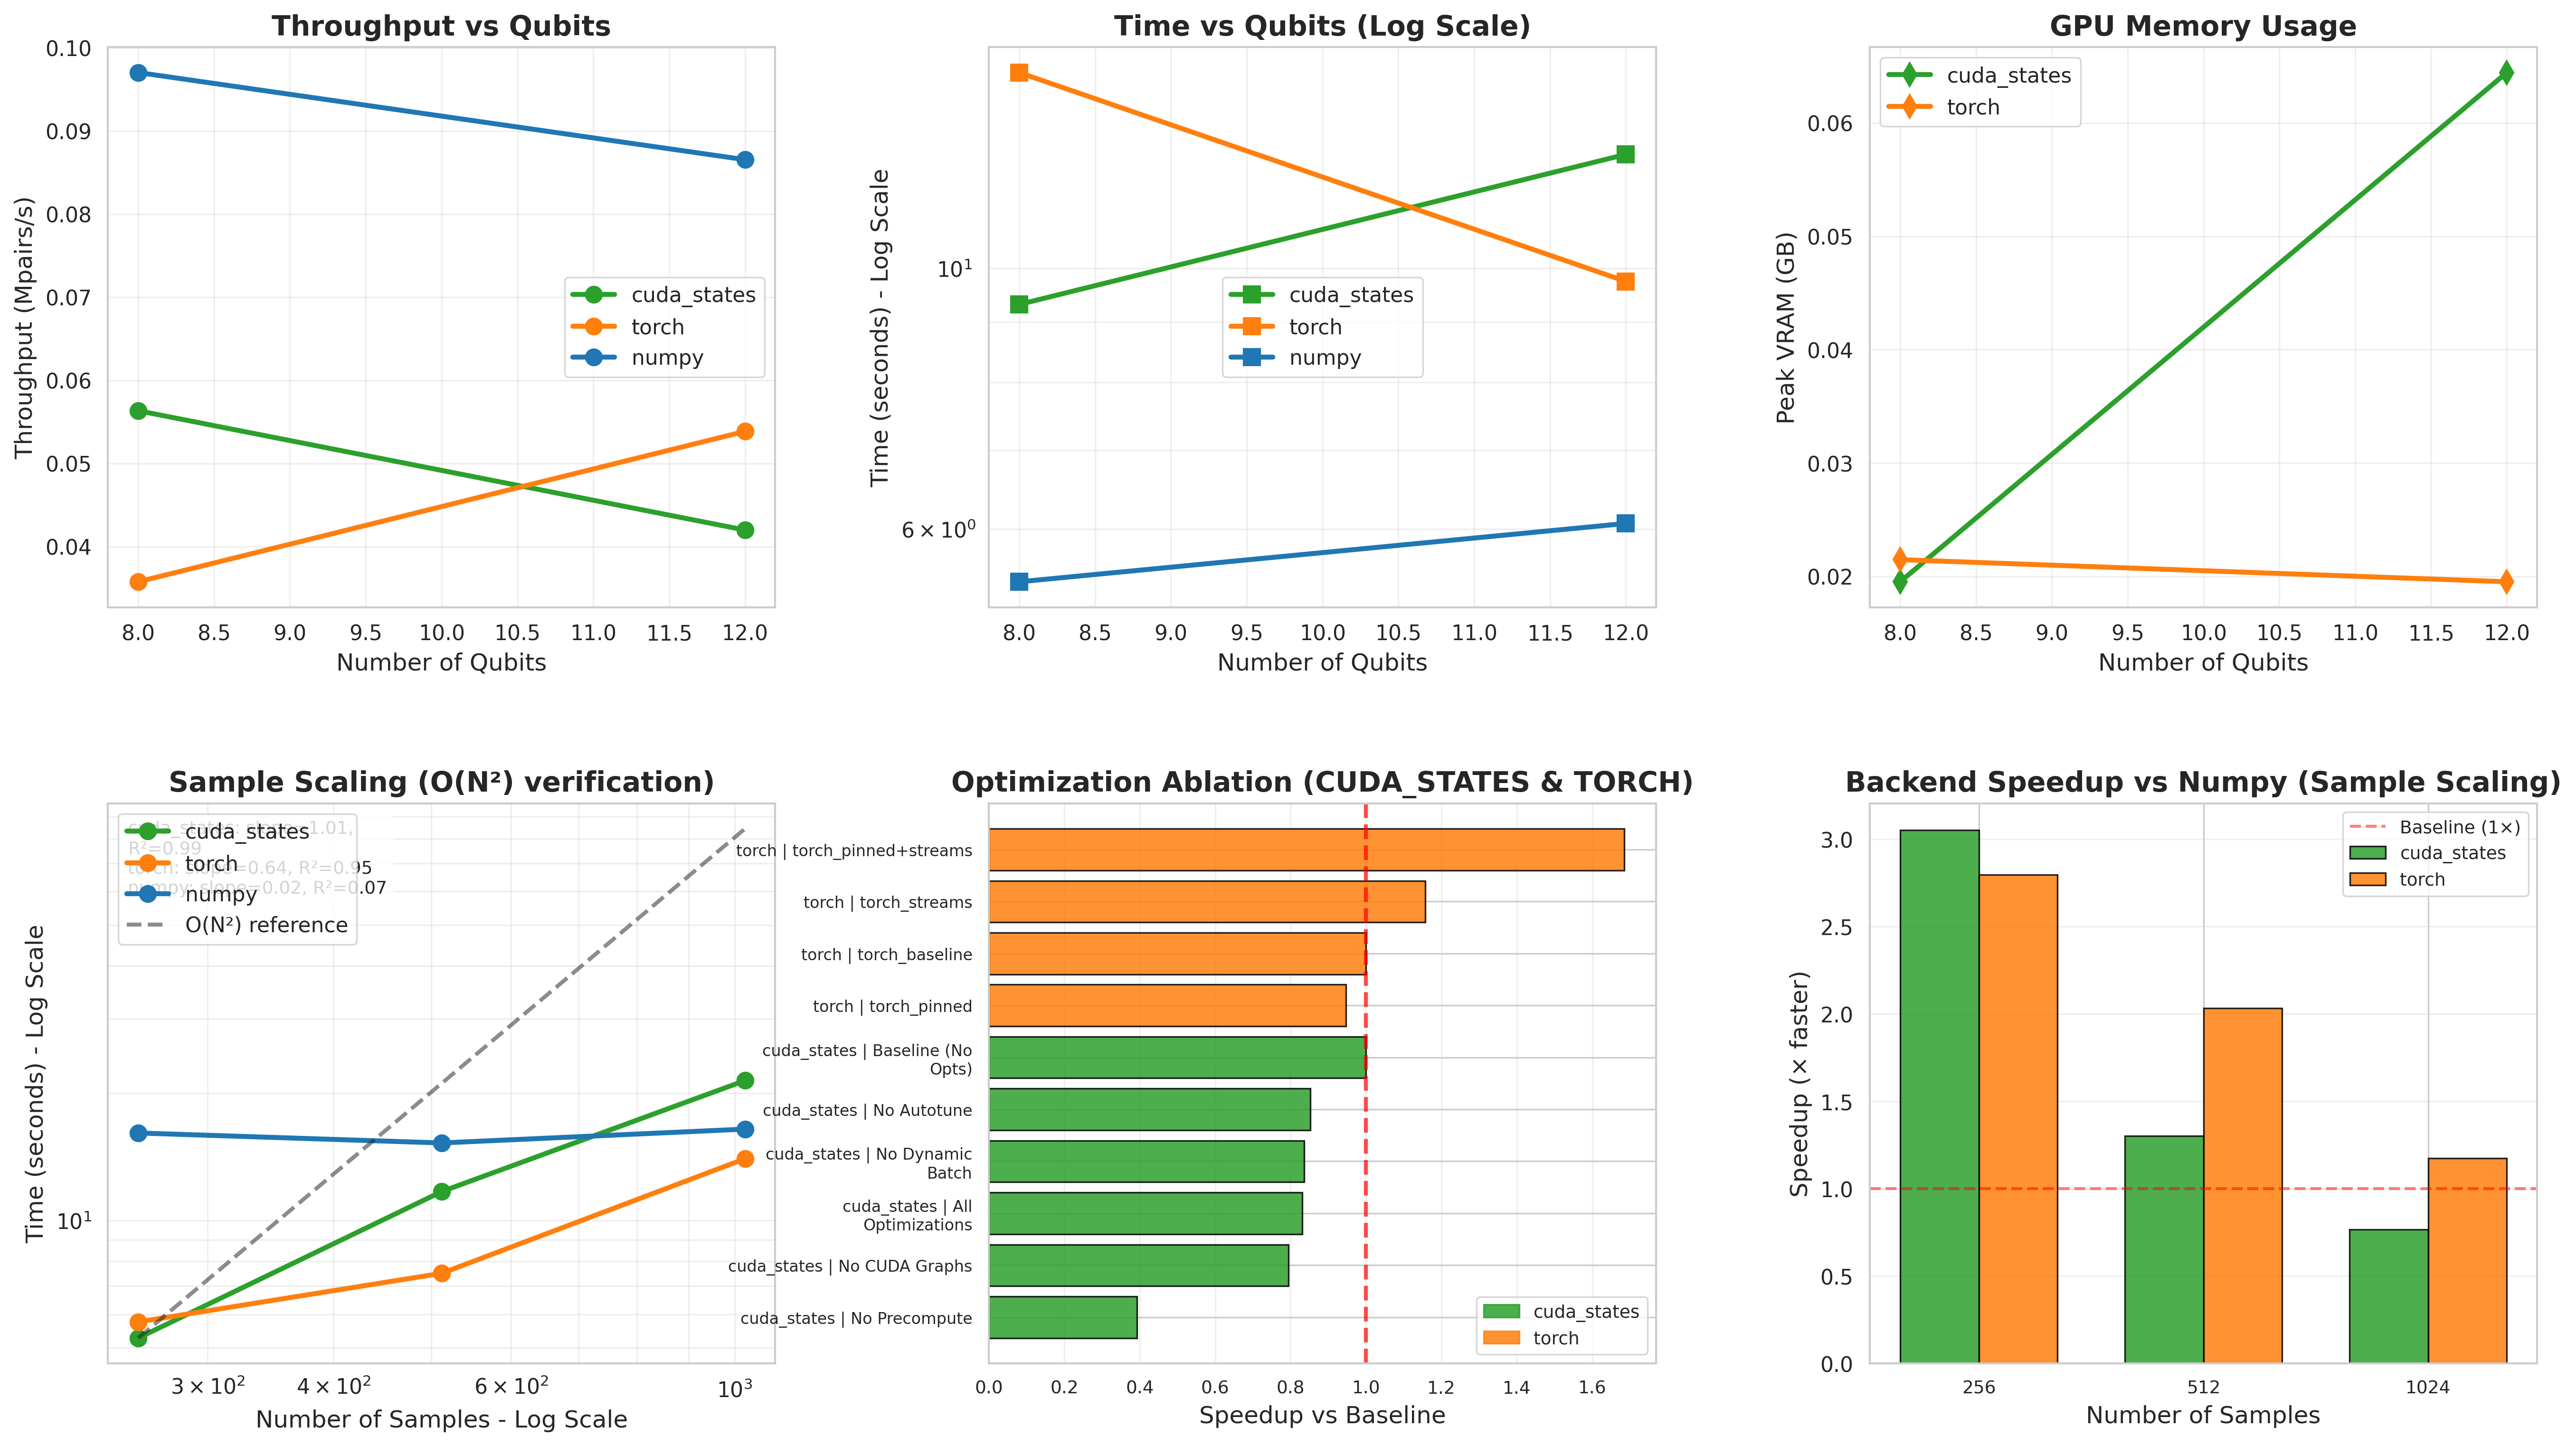
\includegraphics[width=0.92\linewidth]{benchmark_results/cifar10/benchmark.png}
        \captionof{figure}{CIFAR-10 (16 qubits)}
        \column{0.50\textwidth}
        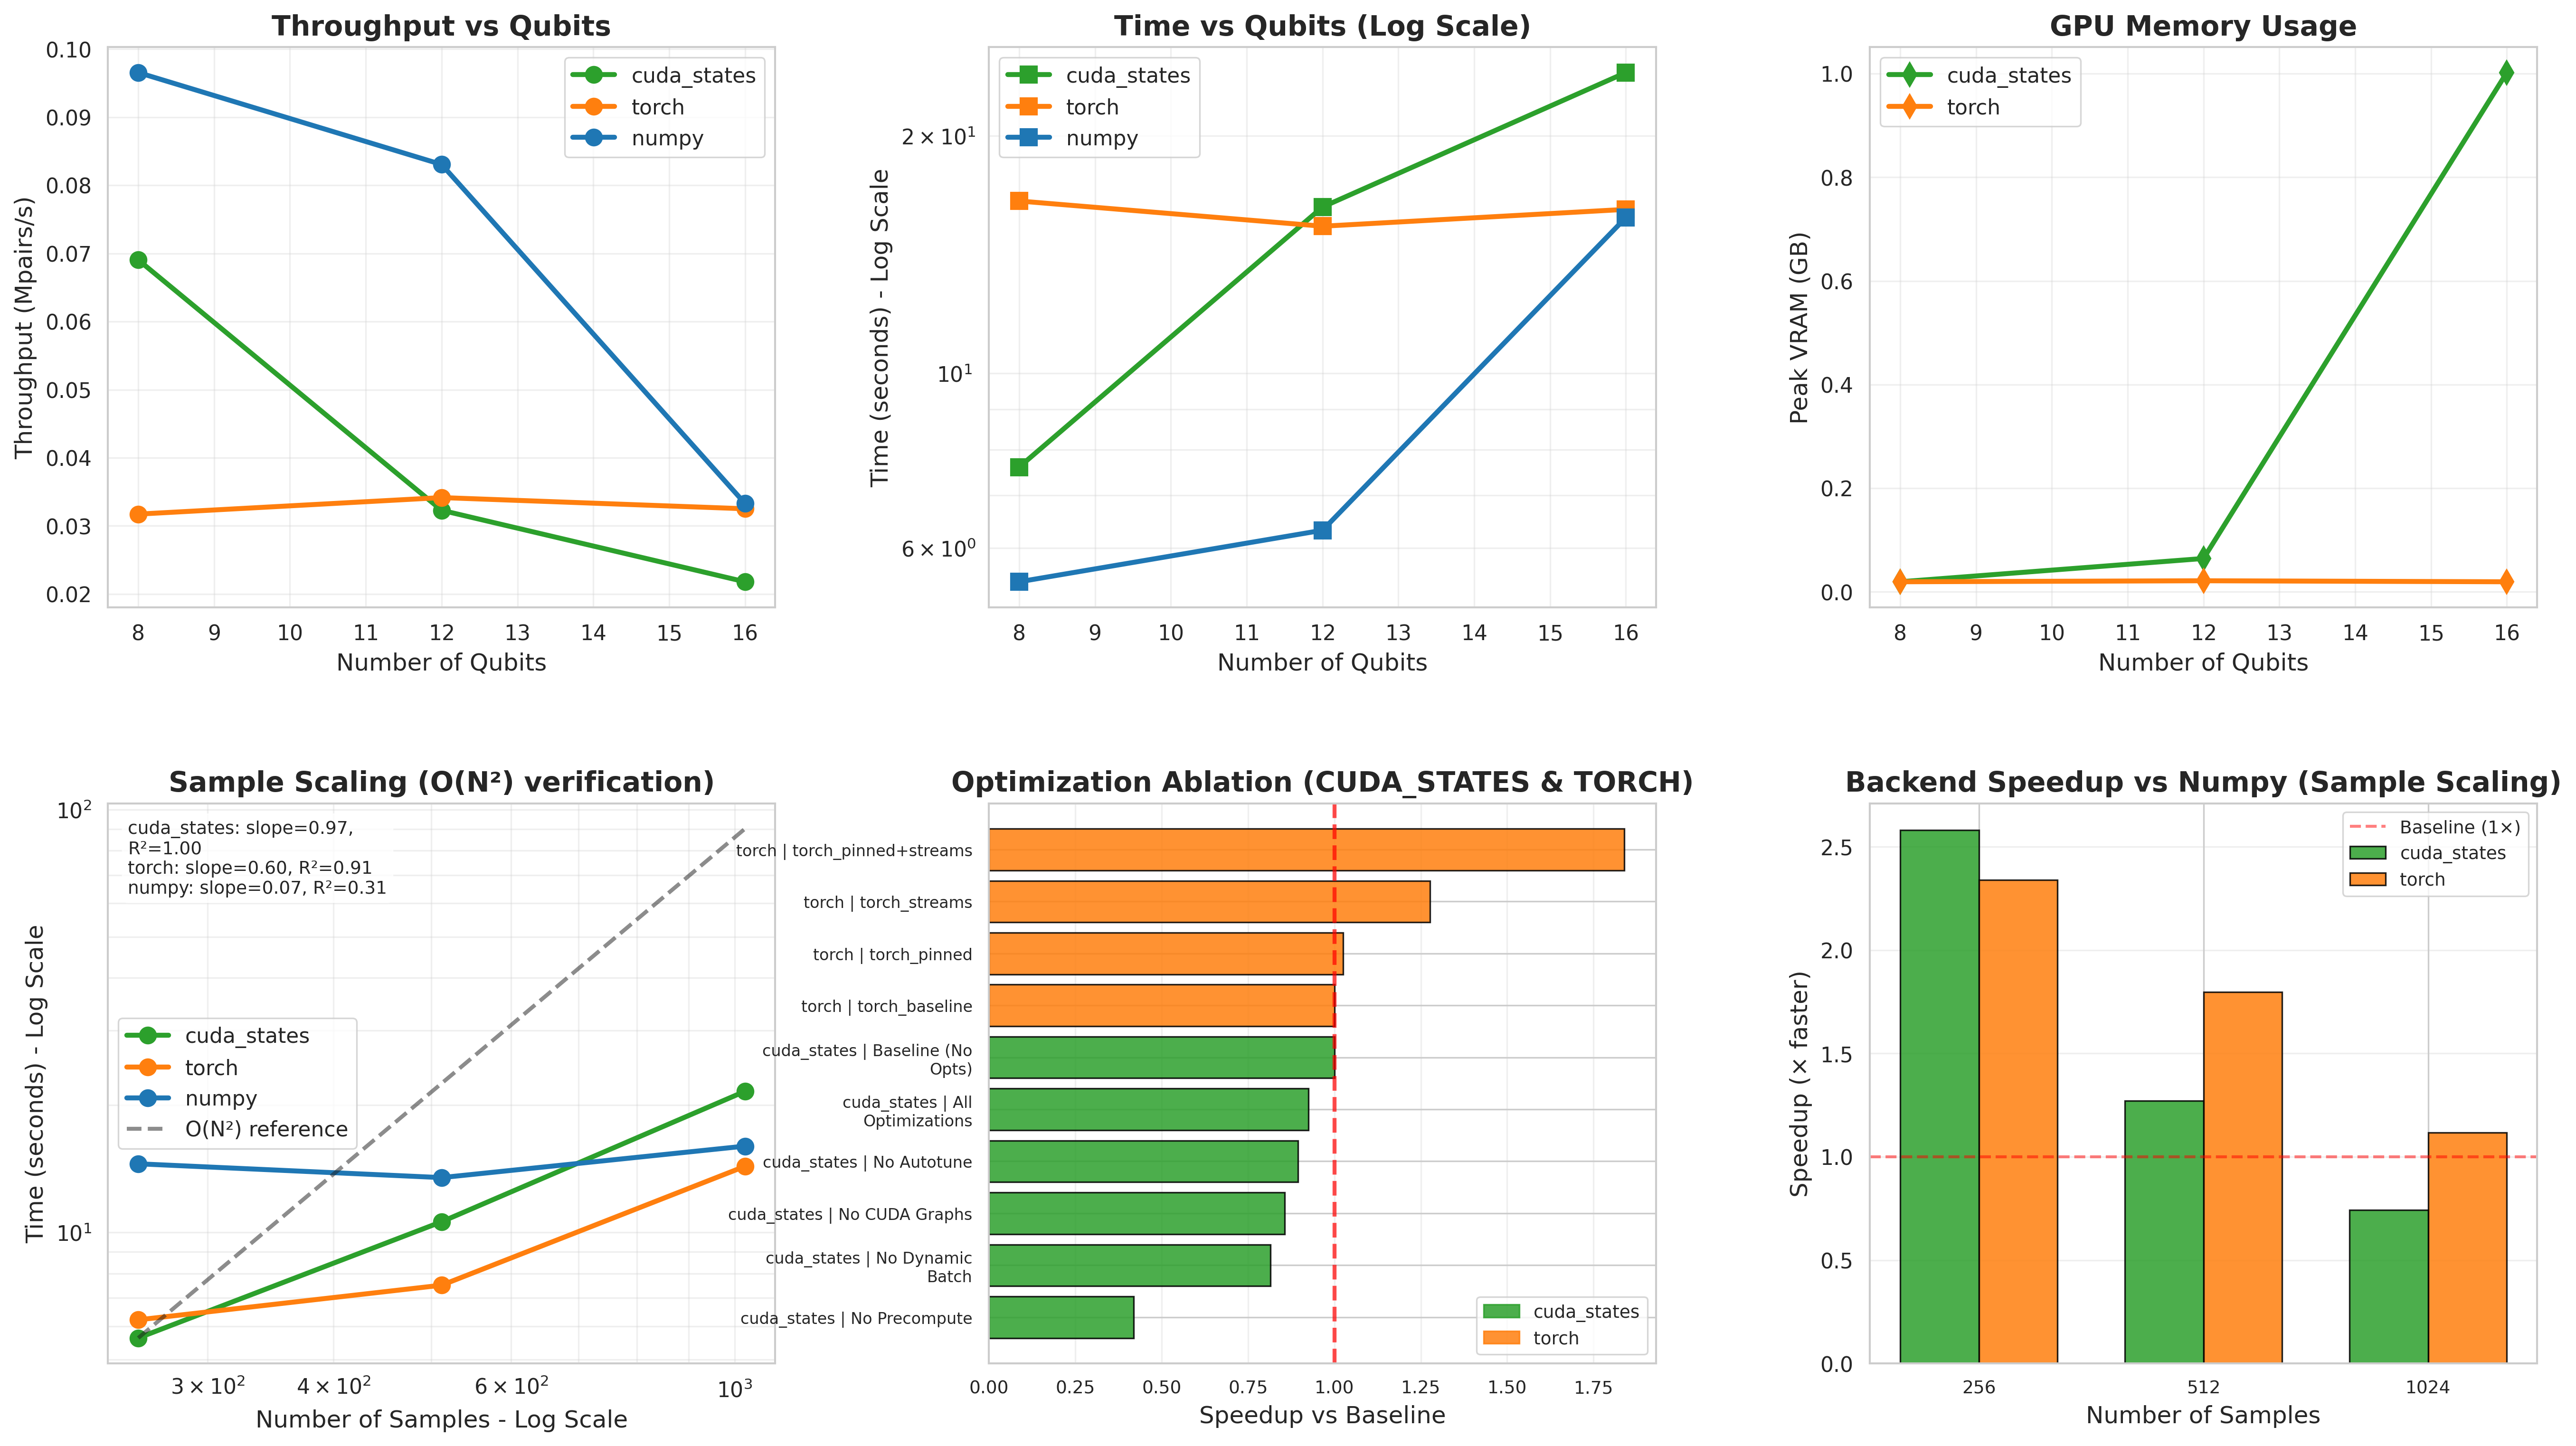
\includegraphics[width=0.92\linewidth]{benchmark_results/svhn/benchmark.png}
        \captionof{figure}{SVHN (16 qubits)}
    \end{columns}
    \vspace{0.1cm}
    {\small GPU base is fastest across most 16-qubit configurations. Data movement dominates over stream complexity.}
\end{frame}

% =========================================================================
\section{Classification Results}
% =========================================================================

\begin{frame}{Quantum Backend Quality vs Runtime}
    \begin{center}
    {\scriptsize Mean F1, AUC and runtime -- averaged over difficulty levels, latest run extraction}
    \end{center}
    \vspace{-0.15cm}
    \begin{center}
    \scriptsize
    \rowcolors{2}{gray!10}{white}
    \begin{tabular}{llcccc}
        \toprule
        \textbf{Dataset} & \textbf{Size} & \textbf{Backend} & \textbf{Mean F1} & \textbf{Mean AUC} & \textbf{Mean time (s)} \\
        \midrule
        cifar10 & 500  & GPU custom & 0.3500 & 0.4480 & 336.13 \\
        cifar10 & 500  & GPU base   & 0.4270 & 0.4812 & 190.61 \\
        cifar10 & 1000 & GPU custom & 0.4305 & 0.4365 & 496.73 \\
        cifar10 & 1000 & GPU base   & 0.5729 & 0.5532 & 302.19 \\
        fashion & 500  & GPU custom & 0.8905 & 0.9569 & 237.05 \\
        fashion & 500  & \textbf{GPU base}   & \textbf{0.8889} & \textbf{0.9574} & \textbf{110.78} \\
        fashion & 1000 & GPU custom & 0.8958 & 0.9553 & 339.29 \\
        fashion & 1000 & \textbf{GPU base}   & \textbf{0.8998} & \textbf{0.9557} & \textbf{187.13} \\
        svhn    & 500  & GPU custom & 0.1789 & 0.4719 & 545.39 \\
        svhn    & 500  & GPU base   & 0.1547 & 0.4719 & 302.73 \\
        svhn    & 1000 & GPU custom & 0.1596 & 0.4846 & 637.30 \\
        svhn    & 1000 & GPU base   & 0.2998 & 0.4846 & 380.61 \\
        \bottomrule
    \end{tabular}
    \end{center}
    {\small \textbf{GPU base} generally faster and more accurate. Fashion strong; SVHN/CIFAR-10 degrade.}
\end{frame}

\begin{frame}{Classical vs Quantum: Paired Comparison}
    \begin{center}
    {\scriptsize Positive $\Delta$F1/$\Delta$AUC = classical better; negative $\Delta$Time = classical faster}
    \end{center}
    \vspace{-0.1cm}
    \begin{center}
    \small
    \rowcolors{2}{gray!10}{white}
    \begin{tabular}{lccccc}
        \toprule
        \textbf{Comparison} & \textbf{Size} & $\Delta$\textbf{F1} & $\Delta$\textbf{AUC} & $\Delta$\textbf{Time (s)} & \textbf{Wins C/T/Q} \\
        \midrule
        Classical $-$ GPU base   & 500  & +0.1708 & +0.1488 & $-$188.28 & 8/0/1 \\
        Classical $-$ GPU base   & 1000 & +0.1721 & +0.1600 & $-$274.52 & 8/1/0 \\
        Classical $-$ GPU custom & 500  & +0.1879 & +0.1600 & $-$359.76 & 8/0/1 \\
        Classical $-$ GPU custom & 1000 & +0.2676 & +0.1990 & $-$475.66 & 8/1/0 \\
        \bottomrule
    \end{tabular}
    \end{center}
    \vspace{0.2cm}
    \begin{itemize}
        \item Classical \textbf{dominates}: wins 8/9 paired comparisons at both sample sizes
        \item Quality gap \textbf{widens at 1000 samples} -- quantum kernels do not scale better with data
        \item Acceleration improves throughput but does \textbf{not remove representational limits}
    \end{itemize}
\end{frame}

% =========================================================================
\section{Failure Analysis: Kernel Collapse}
% =========================================================================

\begin{frame}{Hard Tasks: Quantitative Failure Pattern}
    \begin{columns}[T,onlytextwidth]
        \column{0.50\textwidth}
        \textbf{Observable collapse signals:}
        \begin{itemize}
            \item Inter-class gap $\approx 0$ after normalization
            \item Kernel std $\in [10^{-4},\,10^{-3}]$
            \item SV fraction $\to 1.0$
            \item AUC $\approx 0.5$ (random)
        \end{itemize}
        \vspace{0.3cm}
        \textbf{Hard CIFAR-10 with 6 layers:}
        \begin{itemize}
            \item \textit{kernel std = 0.0005}
            \item \textit{SV frac = 1.0000}
            \item \alert{\textit{test F1 = 0.0000}}
            \item \alert{\textit{test AUC = 0.4757}}
        \end{itemize}
        \column{0.47\textwidth}
        \begin{alertblock}{\faBan\ Kernel Concentration}
            States become nearly \textbf{indistinguishable}. All samples become support vectors -- the SVM cannot separate classes.
        \end{alertblock}
        \vspace{0.3cm}
        \textbf{Contributing factors:}
        \begin{itemize}
            \item PCA/grayscale information loss
            \item Generic ansatz, not image-aware
            \item Deeper circuits $\to$ more concentration
            \item Global fidelity kernel limitation
        \end{itemize}
    \end{columns}
\end{frame}

\begin{frame}{Difficulty-Level Summary Across Backends}
    \begin{center}
    {\small Mean F1, AUC and time per difficulty (averaged over datasets and sizes, latest run)}
    \end{center}
    \vspace{-0.15cm}
    \begin{center}
    \small
    \rowcolors{2}{gray!10}{white}
    \begin{tabular}{lccc}
        \toprule
        \textbf{Difficulty / Backend} & \textbf{F1} & \textbf{AUC} & \textbf{Time (s)} \\
        \midrule
        easy / GPU custom & 0.4907 & 0.6327 & 475.44 \\
        easy / GPU base   & 0.6366 & 0.6499 & 258.76 \\
        med  / GPU custom & 0.5263 & 0.6314 & 404.06 \\
        med  / GPU base   & 0.6560 & 0.6896 & 226.39 \\
        hard / GPU custom & 0.4357 & 0.6125 & 416.44 \\
        hard / GPU base   & 0.3289 & 0.6126 & 251.88 \\
        \bottomrule
    \end{tabular}
    \end{center}
    \vspace{0.2cm}
    \begin{itemize}
        \item \textbf{GPU base} outperforms at easy/med -- faster and more accurate
        \item At \textbf{hard}, both backends collapse: F1 drops, AUC $\to$ 0.5
        \item Compute acceleration cannot resolve the representational bottleneck
    \end{itemize}
\end{frame}

% =========================================================================
\section{Conclusion \& Perspectives}
% =========================================================================

\begin{frame}{Conclusion}
    \begin{itemize}
        \setlength\itemsep{0.85em}
        \item[\faCheckCircle] \textbf{HPC Pipeline:} Three backends share a unified API. GPU paths dominate small sizes; ranking varies with dataset and sample count.
        \item[\faChartLine] \textbf{Fashion quality:} Both quantum backends competitive (F1 up to \textbf{0.9653}, AUC up to \textbf{0.9956} for GPU base, size 1000).
        \item[\faExclamationCircle] \textbf{Classical dominates:} RBF SVM wins 8/9 paired comparisons at both sample sizes. Gap widens at 1000 samples.
        \item[\faBan] \textbf{Kernel collapse on hard tasks:} Concentration signals (std $\sim 10^{-4}$, SV frac = 1). Acceleration alone does not fix this.
    \end{itemize}
\end{frame}

\begin{frame}{Perspectives}
    \begin{columns}[T,onlytextwidth]
        \column{0.48\textwidth}
        \textbf{\faArrowRight\ Better Feature Maps}
        \begin{itemize}
            \item Projected/local kernels to reduce concentration
            \item Geometry-aware ansatz for image structure
            \item Stronger classical front-end before quantum embedding
        \end{itemize}
        \vspace{0.3cm}
        \textbf{\faArrowRight\ Richer Diagnostics}
        \begin{itemize}
            \item Gap trajectories and kernel spectra
            \item SV dynamics to detect collapse earlier
            \item Broader benchmark grids per dataset
        \end{itemize}
        \column{0.48\textwidth}
        \textbf{\faArrowRight\ HPC Scaling}
        \begin{itemize}
            \item Multi-GPU / MPI for large Gram builds
            \item GPU-side SVM solvers to remove CPU bottleneck
        \end{itemize}
    \end{columns}
\end{frame}

\begin{frame}[plain]
    \centering
    \vspace*{0.9cm}
    {\LARGE\textbf{Thank You!}\par}
    \vfill
    {\normalsize\faGithub\ github.com/DylanUnifi\par}
    \vspace{0.30cm}
    {\normalsize\faUniversity\ University of Florence\par}
    \vspace{0.65cm}
    {\large\textbf{Questions?}\par}
    \vspace*{0.9cm}
\end{frame}

\end{document}
